er Begriff Cloud Computing ist laut eines Technology Report bis auf das Jahr 1996 zurückzuführen, wo er in einem Business-Plan des Unternehmens Compaq von ein paar Entwicklern genutzt worden sein sollen, um über die zukünftigen Entwicklungen des Internet-Businesses zu diskutieren \cite{regalado2011coined}.\\\\ 
Auch wenn das Konzept des Cloud-Computings, die dynamische, skalierbare, zuverlässige und unbegrenzte Bereitstellung von Ressourcen als Dienst über das Internet, immer mal wieder in der Literatur auftauchte \cite{fox2009above}, so erlangte es erst ab 2006 einen immer größter werdenden Bekanntheitsgrad. 2006 veröffentlichte AWS das Produkt Elastic Compute Cloud (EC2), gefolgt von Goolges App Engine 2008. Bereits in diesem früher Stadium wurde mit App Engine das Prinzip einer sog. \glqq stateful\grqq{}-Ebene, für das Speichern von des Aktuellen Anwendungsstatus und einer \glqq stateless\grqq{}-Ebene für die Ausführung des eigentlichen Programmes unterschieden \cite{fox2009above}. Des Weiteren wurde 2009 in einer Berkeley-Studie die sechs größten Potentiale des Cloud-Computings herausgearbeitet welche bis heute in den unterscheidlichen XaaS-Konzepten umgesetzt wurden. Im folgenden sind diese kurz auf gelistet. \\
\begin{itemize}
\item[1.] Unbegrenzte Ressourcen wann immer sie benötgt werden. 
\item[2.] Durch die Möglichkeit mit wenigen Ressourcen zu starten, vielen Nutzern zugang zu der Plattform zu gewähren. 
\item[3.] Die genutzen Ressourcen so genau wie möglich nach dem \glqq Pay Per Use\grqq{}-Prinzip zu bezahlen. 
\item[4.] Größenvorteile (Economies of scale) nutzen, um die Kosten durch eine dauerhafte, optimale Ausnutzung riesiger Datencenter auf ein Minimum zu reduzieren. 
\item[5.] Operationelle Kosten so weit es geht zu senken und die Ressourcennutzung durch Virtualisierung so weit wie möglich auszunutzen. 
\item[6.] Eine hohe Hardwareausnutzung durch \glqq Multiplexing\grqq{} der Auslastungen verschiedener Unternehmen zu erreichen.
\end{itemize}
Das National Institute of Standards and Technology (NIST) veröffentlichte 2011, nach 16 vorausgehenden Definitionen, schließlich eine finale Definition des Cloud-Computings, welche bis heute als orientierung Anwendung findet und in einer vielzahl an Werken aufgegriffen wird \cite{mell2011nist}. Die Definition nach NIST beschreibt das Cloud model als eines aus fünf essentiellen Charakteristiken und drei Service Modellen, IaaS, PaaS und SaaS bestehendes Modell, mit insgesamt vier Deployment-Models.\\\\ 
\textit{"Cloud Computing is a model for enabling ubiquitous, convenient, on-demand network access to a shared pool of configurable computing resources (e.g., networks, servers, storage, applications, and services) that can be rapidly provisioned and released with minimal management effort or service provider interaction."} \cite{mell2011nist}.\\\\ 
NIST bricht die Definition mit Essentiellen Charakteristiken, Service-Models und Deployment-Models in drei Unterkategorien herunter, welche erfüllt sein müssen um dem Anspruch an Cloud Computing zu genügen. \\
Grob gefasst sind dies bei den Characteristiken, die automatische Bereitstellung der benötigten Ressourcen je nach bedarf (\textit{On-demand self-service}), die Möglichkeit von allen gängigen Geräten darauf zugreifen zu können (\textit{Broad network access}), die optimale Verteilung von Ressourcen auf die Kunden welche sie gerade benötigen, wobei hier die exakte lokation dieser von geringer Relevanz ist (\textit{Resource pooling}), die automatische Skalierung von Ressourcen (\textit{Rapid elasticity}) und die Möglichkeit der Überwachung und Limitierung der Ressourcenausnutzung, welche für den Kunden als auch den Anbieter transparent sein muss (\textit{Measured service}).\\\\ 
Bei den Service Models werden hier lediglich IaaS, PaaS und SaaS unterschieden. Laut NIST gibt es um den Code in der Could bereitzustellen vier verschiedene Deployment-Models, welche genutzt werden können. Mit der \textit{Private cloud}, obliegt es dem Unternehmen seine Infrastruktur komplett selber zu betreiben, jedoch muss diese dem Unternehmen dabei nicht selber gehören, sondern kann von eine dritten Partei gehostet werden. Mit dem deployment auf eine \textit{Community cloud} teilen sich verschiedene Unternehemen eine Cloud, welche entweder von ihnen gemeinsm, oder von einem Drittanbieter betrieben wird. Zuletzt gibt es noch die Möglichkeit die von einem Cloud-Computing-Anbieter bereitgestellte öffentliche Cloud \textit{Public cloud} zu nutzen, bei welcher das Unternhemen die Räumlichkeiten bzw. Ressourcen von einem Dittanbieter nutzt. Das letzt Deployment-Model stellt die sog. \textit{Hybird cloud} dar, welche eine Kombination aus den vorherigen darstellt \cite{mell2011nist}.
\subsection{Abwägung zwischen Open-Source und Cloud-Vendor}
% Wie bereits im vorherigen Abschnitt beschrieben, 
% OpenFaaS  
Die Abwägung zwischen der Implementation von Function as a Service in der unternehmenseigenen Cloud bzw. Servern oder dem Outsourcen an einen proprietären Cloud-Vendor, sollte wohl überlegt sein, da hiervon in der Folge eine Vielzahl an Möglichkeiten und Restriktionen abhängt. \\\\
Entscheidet man sich für ersteres, also dem Aufbau einer privaten FaaS-Plattform so stehen hierfür, mit IBM Apache OpenWhisk, Fission, OpenFaaS oder Kubless, nahezu identisch viele Frameworks zur Verfügung wie bei den öffentlichen Vendoren. \textcolor{blue}{Schaubild CNCF Serverless Landscape ggf. einfügen.} Des Weiteren bietet dieser Weg, abgeseh en von der Vielfalt an Frameworks mit wiederum unterschiedlichen Eigenschaften, die Möglichkeit die Größe der Funktionen oder die maximal zulässige Laufzeit eines Containers individuell anzupassen. Dies würde einerseits eine granularer Verrechnung der in Anspruch genommenen Ressourcen der einzelnen Bereiche oder Teams zulassen, zugleich aber auch ein Operations-Team verlangen, welches sich in das jeweilige Framework einarbeitet, die Plattform zu dessen Betrieb aufsetzt und die spätere Wartung dieser übernimmt. \cite{mohanty2018evaluation}.\\\\
Eine Alternative stellen proprietäre Lösungen von öffentlichen Cloud-Vendoren, wie beispielsweise Amazon Web Services (AWS) Lambda, Microsofts Azure Functions, IBM Cloud Functions oder Google Cloud Functions, bei welchen sich von Unternehmensseite aus niemand um die Wartung der Infrastruktur, die Skalierung der Services, die Behandlung von Fehlermeldungen o.ä. kümmern muss. Diese Aufgaben werden in der Folge von dem Plattformbetreiber übernommen. Natürlich sind diese Dinge in erster Linie Aufgabe des Plattformbetreibers, jedoch haben sie unmittelbare Auswirkungen auf das Unternehmen, sollten Probleme beim Skalieren von Funktionen oder dem Monitoring auftreten. Sollte dies der Fall sein, so sind die Entwickler von den bereitgestellten Debugging Möglichkeiten und Monitoring-Lösungen der Plattform abhängig um Probleme schnellstmöglich zu beheben, sollte dies die Plattform nicht tun. Daneben ist ein weiterer Punkt des Vendor Lock-Ins die von Anbieter zu Anbieter variierende Infrastruktur, welche ein einfaches Shiften von Funktionen erheblich erschwert. Zudem sind die Benutzung der Funktionen meist automatisch mit der Inanspruchnahme weiterer Services der Plattform, wie dem Message Queuing oder der Datenspeicherung, gekoppelt. \\\\
Dies hat sowohl Vor- als auch Nachteile. Ist man bei der Einrichtung der privaten FaaS-Cloud auf die unternehmensinternen Ressourcen beschränkt, so bieten die Cloud-Anbieter, neben den Restriktionen des Vendor Lock-Ins, in den meisten Fällen ein großes Ökosystem an weiteren Services, welche sich problemlos an die Funktionen anbinden lassen. Im Folgenden wird daher, auch wenn sich diese Arbeit hauptsächlich auf FaaS beschränkt, das Ökosystem der einzelnen Cloud-Anbieter kurz betrachtet, um einen besseren Überblick über deren zusätzliche Leistungen zu erhalten und eine fundierte Entscheidung treffen zu können.
\cite{lopez2018comparison} hat diese drei Frameworks genuaer untersucht und bei der sequentiell und parallele Planung sowie der Weitergabe des \textit{States} der drei Orchestrierungs-Tool erhebliche Unterschiede feststellen können. Vorab soll an dieser Stelle vermerkt werden, dass nur \glqq warme\grqq{} Instanzen für jegliche nachfolgende Tests genutzt wurden, um Ungenauigkeiten, durch variierende \textit{Cold-Start} Zeiten [siehe \cite{manner2018cold} und \cite{jackson2018investigation}], vorzubeugen.\\\\
In Bezug auf die Ausführung von aufeinander folgenden Funktionen, sequentielle Verarbeitung, erwiesen sich IBM's Composer und ASF als deutlich schneller im Vergleich zu ADF. So Betrug der Overhead, also die Zeit welche nicht zur Ausführung der Funtkion verwendet wurde, bei 40 hintereinander geschalteten Funktionen 1,1s für IBM Composer und 1,2s für AWS Step Functions. Azure Durable Functions brauchten hingegen für die selben 40 Funktionen ganze 8s. Bei weiteren Durchführungen mit [5, 10, 20, 40, 80] stellte sich jedoch heraus, dass IBM Composer die Orchestrierung von Funktionen nur bis zu einer Anzahl von 50 Stück unterstützt. Alles was darüber hinausgeht, müsste durch Orchestrierungs-Tool von Drittanbietern übernommen werden \cite{lopez2018comparison}. ADF und ASF sind wiederum in der Lage \textit{Workflows} festzulegen, welche über Tage und Monate lauffähig sind.\\\\
Die Evaluierung des Overheads bei parallel geschalteten Funtkionen wurde für ASF und ADF durchgeführt. Dabei wurde wieder mit 5 Funktionen begonnen und sich, wie oben beschrieben, bis auf 80 hochgearbeitet. Die Ergebnisse waren eindeutig. Bei einer Anzahl von 80 Funktionen hatten Azure Durable Functions mit einem durchschnittlichen Overhead von 32.1s fast das doppelte Volumen von AWS Step Functions mit einem durchschnittlichen Overhead von 18.3s. Die Ergbenisse legten zudem nahe, dass ASF zuverlässiger bei der Vorhersage des zu erwatenden Overheads ist als ADF. Microsofts Overhead stieg nicht immer gleichbleibend exponentiell an wie der von Amazon, was eine Prognose über das Verhalten erschwert.\\\\
Bei der Evaluierung für die Eignung von parallel geschalteten Funktionen viel IBMs Composer direkt zu Beginn aus dem Testportfolio heraus, da parallele Ausführungen nicht unterstützt wurden [stand 2018 \cite{lopez2018comparison}]. Mittlerweile [stand 2020] wird von Seiten IBMs die parallele Ausführung von Funktionen seitens Composer zwar unterstützt und gesagt, dass seitens Composer dies nicht auf eine bestimmte Anzahl von Funktionen beschränkt ist\footnote{https://github.com/apache/openwhisk-composer}. Allerdings wird explizit erwähnt, dass eine Limitierung gleichzeitig ausführbarer Funktionen Seitens OpenWhisk besteht, welche bei Überschreitung zu Fehlern führen kann: \glqq [...] many concurrent invocations may hit OpenWhisk limits leading to failures: failure to execute a branch of a parallel composition or failure to complete the parallel composition [...]\grqq{}\footnote{https://github.com/apache/openwhisk-composer}. Die derzeitige Limitierung gleichzeitiger Funktionen in OpenWhisk liegt bei 100 pro \textit{Namespace}\footnote{https://github.com/apache/openwhisk/blob/master/docs/}.\\\\
Zuletzt wurden die drei Orchestrierungs-Lösungen bezüglich der Weitergabe des \textit{Application-States} untersucht. Aufgrund der Begrenzung von ASF auf 32KB wurde bei den beiden anderen Lösungen die selbe Größe gewählt. Dieses mal wurden nur 5 sequentiell ablaufende Funktionen getestet. Die Grenze bei IBM Cloud Functions lag 2018 offiziell bei 1MB, liegt mittlerweile aber bei 5MB\footnote{https://cloud.ibm.com/docs/openwhisk?topic=cloud-functions-limits}. ADF hingegen ermöglich die Weitergabe von bis zu 60KB. Es zeigte sich, dass IBM Composer und AWS Step Functions bei der Ausführung ohne \textit{Payload}, jeweils einen Overhead von 175.7ms und 168.0ms hatten. Mit Payload betrug der Overhead in ms für Composer 298.4 und Step Functions 287.0, was eine Zunahem von 70\% darstellt [siehe Abbildung ~\ref{fig:orchestration}]. Azure Durable Functions stieß bei diesem Test deutlich hervor. Mit einem Overhead von 766.2ms ohne Paylod und 859.5ms mit Payload ist der grundlegende Overhead zwar deutlich höher als bei den beiden vorherigen, steigt unter Last aber nur um 12\% an \cite{lopez2018comparison}.
\begin{figure}[H]
    \caption{Overhead bei 5 sequentiellen Funktionen mit einem Payload von 32KB, nach \cite{lopez2018comparison}}
    \label{fig:orchestration}
    \centering
    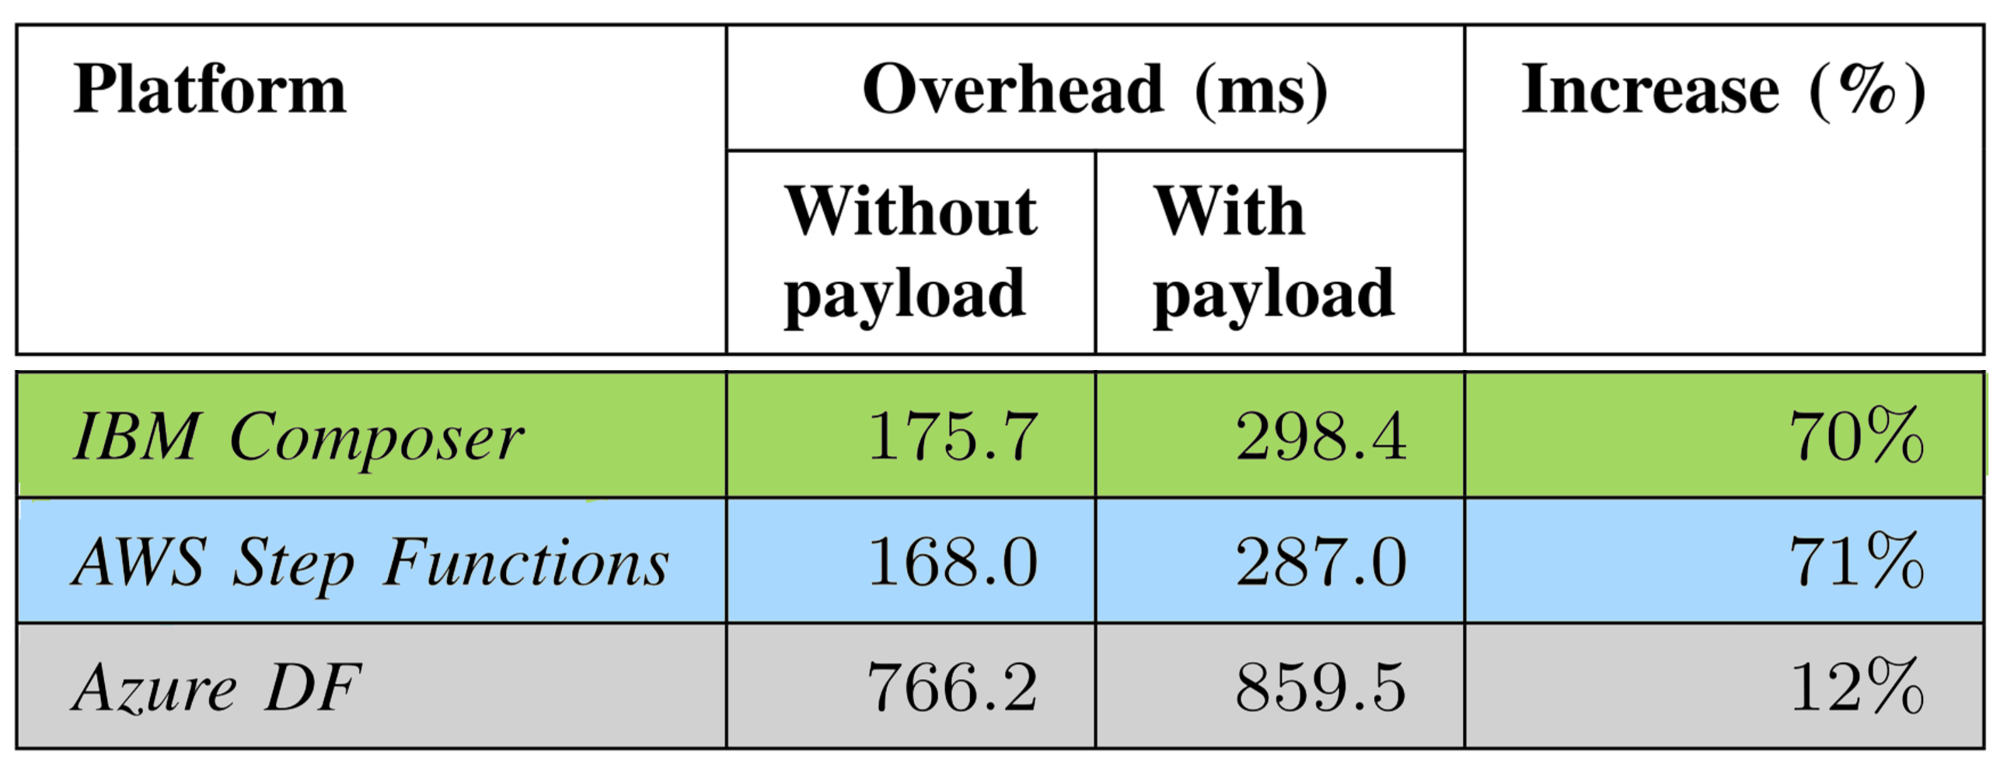
\includegraphics[width=0.7\textwidth]{Orchestration}
    \end{figure} 

Anhand der durch Lopez et al. gezeigten Ergebnisse lässt sich festhalten, dass AWS mit Step Funtion das ausgereifteste Orchestrierungs-Tool zur Verfügung stellt. Sowohl bei der sequentiellen als auch bei der parallelen Ausführung beitet AWS Lösungen für langlebige und kurzlebige Funktionskopplungen. Zudem ermöglicht die Limitierung des \textit{States} auf 32KB eine klare auskunft über die entstehenden Kosten zu geben. Hat man vor FaaS lediglich für leichtgewichtige Aufgaben zu nutzen, so spielt IBM Composer bei der Kopplung von bis zu 50 Funktionen seine Stärken aus und ist dabei geringfügig schneller als AWS. Für die Festlegung längerer Abläufe, welche auf das Laufen über Tage bis hin zu Monaten ausgelegt sind, ist Composer nicht geeignet \cite{lopez2018comparison}. Steht der Austausch des \textit{Application-States} zwischen Funktionen im Vordergrund und können höhere Latenzzeiten in Kauf genommen werden, bietet Azure mit einer Kapazität von 60KB eine Alternative zu AWS und IBM. Auch Abläufe die länger Zeit beanspruchen können mit ADF konfiguriert werden. Das Konzept von \textit{async/await} bei sequentiellen und \textit{fan-out/fan-in}\footnote{https://docs.microsoft.com/en-us/azure/azure-functions/durable/durable-functions-cloud-backup} bei parallelen Abläufen bietet zusätzlich eine etwas leichtere Umsetztung als AWS und IBM \cite{lopez2018comparison}.


\subsection{Auswirkungen auf die Testumgebungen}
Zum Testen einer serverlosen Applikation stehen mehrere Möglichkeiten zur Verfügung, welche ihre Vor- und Nachteile haben. Unterschieden wird in lokales Unit-Testen, Canary Release Testen ing sowie A/B Testen und Integrationstests. War OpenWhisk zu Beginne einer der ersten Anbieter, welcher lokale Unit-Tests unterstützte, so zogen AWS mit SAM\footnote{$https://aws.amazon.com/de/serverless/sam/?nc1=h_ls$} und Azure mit seinen sog. Function Core Tools\footnote{https://docs.microsoft.com/en-us/azure/azure-functions/functions-develop-local} nach. In diesen Unit-Tests liegt jedoch bereits eine Einschränkung, die bei der Migration bedacht werden muss. Gibt es bei Anwendungen die nicht über einen \textit{Serverless Cloud-Provider} laufen oft die Möglichkeit Teile der Anwendung durch lokale Kopien von Datenbanken oder Message-Queues, welche denjenigen in der Produktion sehr ähnlich sind, bi dem Testen zu integrieren, so ist dies bei serverlosen Funktionen schwerer \cite{roberts2017serverless}.  Dadurch, dass die Funktionen in den meisten Fällen mit anderen Funktionen sowie Datenbanken und ggf. noch einigen weiteren Services des Anbieters interagieren müssen, ist es nicht möglich dies lokal zu simulieren, zumal in der Plattform gesetzte Konfigurationen lokal nicht umgesetzt werden können. Kennzahlen wie die Ausführungszeit von Funktionen, das Laden von Abhängigkeiten (Libraries) und Verzögerungen durch \textit{Cold-Starts} können nicht akkurat wiedergegeben werden \cite{racicot2019quality}. Mit der Abgabe der Hoheit über die Infrasturktur kann hinzukommend auch nicht mehr der Server bestimmt werden, auf dem die Funktion letzten Endes gestartet wirde, was im zweifel, bei älterer Hardware, die Ausführungszeit der Funktion erhöhen kann. Es ist daher unumgänglich den Service auch auf der Plattform selber zu testen, um zuverlässige Daten über Perfomanz und Kompatibilität zu erhalten.\\\\ Eine Möglichkeit hierfür bietet das sog. Canary-Testen, bei welchem es nicht erforderlich ist die komplette Servicelandschaft auf einen DEV-Account zu spiegeln, später mehr dazu. Stattdessen wird eine neue Version einer bereits existierenden Funktion in Produktion geladen und nur ein bestimmter Teil der Nutzer bzw. Tester darauf umgeleitet. In AWS, sowie bei anderen Anbietern, ist dies bereits in der CLI umgesetzt. Bei AWS wird der vorgang durch etweder \textit{aws-lambda-deploy} oder Sep functions umgesetzt. In der Praxis werden \textit{Canary-Testing} sowie \textit{A/B-Testing} aber nicht sehr häufig durchgeführt \cite{leitner2019mixed}, da dies negative Auswirkungen auf die Performance der in Produktion laufenden Anwendung haben kann. Vor allem Lasttests können dafür sorgen, dass es zu spürbaren Latenzen bis hin zu Ausfällen bei den Nutzern kommt.\\\\ Es bietet sich daher an, den Aufwand einer Spiegelung zu betreiben, da so die in Produktion laufenden Funktionen nicht von Tests beeinflusst werden. Viele Anwender haben dies bereits umgesetzt und es scheint sich als \glqq Best Practice\grqq{} plattformunabhängig etableiert zu haben \cite{leitner2019mixed}. An sich ist dies jedoch nicht verwunderlich, da FaaS bzw. Serverless bei diesem Vorgehen seine Stärken ausspielen kann. So ist es preislich unabhängig, ob das Service-Ökosystem inkl. Funktionen gespiegelt wird oder die Test neben den in Produktion genutzten Funktionen durchgeführt werden. Das Pay-Per-Use-Modell bleibt hiervon unbeeinflusst.    



% Fig. 17. Testing approaches for FaaS functions. tions, but are also determined by what languages are made avail able. For example, of the 8 responses marked ”Other” in Fig. 16 , 5 include ”Go”, which became available in Google’s FaaS offering only when our survey was already live. Development challenges. Given the relative immaturity of the tech nology, it is unsurprising that we have observed some challenges and grievances that even advanced practitioners currently struggle with. A major challenge is how to test functions. Due to the rela tively small size and often low complexity of individual functions, they lend themselves well for unit tests, which can be performed locally. However, testing the integration of multiple functions or external services is harder, as local replication of the entire system is often not possible or hard to achieve. “[... ] it is not possible to replicate a serverless or cloud system on your local machine.” I6. One possible solution is to test functions directly in production, or in a dedicated development environment that is also hosted in the cloud. One common way to implement the latter is to have multiple separate accounts with the cloud provider, one for pro duction and one for development and testing. Both approaches have the obvious disadvantage that they require developers to pay for test invocations the same as for production workload. In ad dition, we have observed that testing in actual production envi ronments can have (negative) side-effects on production systems in some cases. One approach to deal with this issue is to perform canary releases or A/B testing, so that possible side-effects can be assessed for a small number of requests. The testing practices used by survey respondents are illustrated in Fig. 17 . As expected, unit tests are commonly performed locally. When it comes to integration tests, dedicated development envi ronments and mocked environments are more commonly used for testing than production environments (in general, or via canary re leases or A/B tests). 23.7\% (22) of respondents to this question per form tests in both, dedicated FaaS development environments and mocked FaaS environments, while only 16.1\% (15) respondents test both in a dedicated environment (dev or mocked) and in a produc tion environment. nother ore challenge is a lack of tooling and insufficient documentation. Tooling is especially desirable for the interviewees when it comes to deploying (sets of) functions, mapping events to functions (using, for example, API gateways to make functions accessible to HTTP requests), and monitoring and logging. At the same time, only a few of the available tools are actually used. With 79.7\% of survey respondents using it, the Serverless framework is by far the most common among them. Contrary, the next frequently named library, Chalice, was only named by 11.6\% of respondents. This indicates that existing tooling, with the exception of the Serverless framework, appear to not address the core challenges that developers currently face, or their existance is not yet widely known. Fig \cite{leitner2019mixed}



%The orchestration component defines the sequence of tasks; all executions are automatically triggered, each step is tracked and retried in the case of error \cite{werner2018serverless}. AWS Step Functions Each step of an application is triggered, tracked and even retried when errors occur, assuring that applications execute as expected and in the correct order. To aid debugging and diagnostics, logs are kept for every step of the process. Figure 3 shows this process. An added benefit is that step functions can be created and deployed in code through the definition of a state machine using Amazon’s JSON-based States Language10. \cite{werner2018serverless}.


% Kein garantie, dass der folgende Funktionsaufruf auf die selbe bereits laufende Instanz einer Funktion trifft, welche dann wiederum auch zugriff auf dem im Memory gespeicherten State hat. Es ist daher notwendig, dass der Application-State extern gespeichert wird. Auf diesen sog. "\textit{Shared memory}" müssen in der Folge alle Funktionen drauf zugreifen, wenn Applikations-Daten benötigt werden.


% no access to the underlying OS and install agent or daemon to gather metrics isn’t possible. 
% Moreover, the serverless function cannot be used to do some actions after the request is processed, all actions should be finished before returning response because the container is suspended as soon as a response is Moreover, the serverless function cannot be used to do some actions after the request is processed, all actions should be   before returning response because the container is suspended as soon as a response is returned. Therefore, monitoring increases request time. Asynchronous monitoring is possible by-passing metrics as log message and afterward process logs and sends metrics. Such an approach does not prolong requests however it adds delay to monitoring, increases costs due to additional logs processing and increases concurrently executed functions. Maximum limit of concurrently executed functions can be reached faster due processing of logs. Therefore, it’s better to use third-party service, such as Datadog15, when complex log analysis is needed. 
% When incorporating an open surce framework, anotehr layer will be added to the environment to display the different solutions. metrics, change provider when one has too many probelems.


Ein weiterer Punkt bei der Migration von Teilen einer besehenden Architektur, in diesem Fall einer Microservice Architektur, ist die von dem Cloud-Vendor zur Verfügung gestellte Möglichkeit der Orchestrierung der Funktionen. Diese entscheidet darüber wie performant die Funktionen parallel ausgeführt werden können und wie groß der Runtime-Overhead der jeweiligen Plattformen dabei ist. Zudem spielt der Preis der hierfür anfällt eine nicht unerhebliche Rolle, da die sequentielle als auch die parallele Ausführung von Funktionen bei mittleren und großen Softwareprojekten häufig auftreten.\\\\
Wie bereits in \textit{Potentiale und Herausforderungen} unter \textit{Statelessness} erwähnt spielt bei der Kopplung von Funktionen die Weitergabe des Anwendungs- bzw. Funktions-\textit{States} und dessen Geschwindigkeit eine wichtige Rolle. Nur durch das richtige Zusammenspiel vieler Funktionen ist es möglich große Anwendungen zu bauen und komplexe Abläufe umzusetzen. Bei der Betrachtung der unterschiedlichen Hosting-Lösungen soll der Fokus auf die beiden am häufigsten genutzen proprietären FaaS-Lösungen \cite{leitner2019mixed}, AWS Lambda mit Amazon Step Functions und Microsoft Azure Functions mit Azure Durable Functions, gelegt werden. Die Seite der Open-Source Lösungen wird von IBM OpenWhisk, mit IBM Composer als Orchestrierungs-Lösung, vertreten.\\\\



Das National Institute of Standards and Technology (NIST) veröffentlichte 2011, nach 16 vorausgehenden Definitionen, schließlich eine finale Definition des Cloud-Computings, welche bis heute als orientierung Anwendung findet und in einer vielzahl an Werken aufgegriffen wird [MG+11]. Die Definition nach NIST beschreibt das Cloud model als eines aus f¨unf essentiellen Charakteristiken und drei Service Modellen, IaaS, PaaS und SaaS bestehendes Modell, mit insgesamt vier Deployment-Models. ”Cloud Computing is a model for enabling ubiquitous, convenient, on-demand network access to a shared pool of configurable computing resources (e.g., networks, servers, storage, applications, and services) that can be rapidly provisioned and released with minimal management effort or service provider interaction.” [MG+11]. NIST bricht die Definition mit Essentiellen Charakteristiken, Service-Models und DeploymentModels in drei Unterkategorien herunter, welche erf¨ullt sein müssen um dem Anspruch an Cloud Computing zu genügen. Grob gefasst sind dies bei den Characteristiken, die automatische Bereitstellung der benötigten Ressourcen je nach bedarf (On-demand self-service), die M¨oglichkeit von allen g¨angigen Geräten darauf zugreifen zu k¨onnen (Broad network access), die optimale Verteilung von Ressourcen auf die Kunden welche sie gerade benötigen, wobei hier die exakte lokation dieser von geringer Relevanz ist (Resource pooling), die automatische Skalierung von Ressourcen (Rapid elasticity) und die M¨oglichkeit der Uberwachung und Limitierung der Ressourcenausnutzung, welche f¨ur den Kunden als auch den Anbieter transparent sein muss (Measured service). Bei den Service Models werden hier lediglich IaaS, PaaS und SaaS unterschieden. Laut NIST gibt es um den Code in der Could bereitzustellen vier verschiedene Deployment-Models, welche genutzt werden k¨onnen. Mit der Private cloud, obliegt es dem Unternehmen seine Infrastruktur komplett selber zu betreiben, jedoch muss diese dem Unternehmen dabei nicht selber gehören, sondern kann von eine dritten Partei gehostet werden. Mit dem deployment auf eine Community cloud teilen sich verschiedene Unternehemen eine Cloud, welche entweder von ihnen gemeinsm, oder von einem Drittanbieter betrieben wird. Zuletzt gibt es noch die Möglichkeit die von einem Cloud-Computing-Anbieter bereitgestellte öffentliche Cloud Public cloud zu nutzen, bei welcher das Unternhemen die Räumlichkeiten bzw. Ressourcen von einem Dittanbieter nutzt. Das letzt Deployment-Model stellt die sog. Hybird cloud dar, welche eine Kombination aus den vorherigen darstellt [MG+11].




Das National Institute of Standards and Technology (NIST) ver¨offentlichte 2011, nach 16 vorausgehenden Definitionen, schließlich eine finale Definition des Cloud-Computings, welche bis heute als orientierung Anwendung findet und in einer vielzahl an Werken aufgegriffen wird [MG+11]. Die Definition nach NIST beschreibt das Cloud model als eines aus fünf essentiellen Charakteristiken und drei Service Modellen, IaaS, PaaS und SaaS bestehendes Modell, mit insgesamt vier Deployment-Models

Function  as  a  Service  (FaaS)  ist  ein  sogenanntes”Serverless“  Cloud-Computing  Konzept,welches erstmals 2014 von AWS mit Lambda Functions als Preview Release und schließlich2015 zur kommerziellen Nutzung zur Verf ̈ugung gestellt wurde1.  Es kann nach IaaS und PaaSals ein weiterer Schritt in der Entwicklung des Cloud Computings gesehen werden, welcherdas Management von Infrastruktur, Servern und Ressourcen weg von dem Entwickler nimmtund hin zu dem Cloud-Anbieter delegiert.  Ein knappes Jahr sp ̈ater, 2016, traten Microsoftmit Azure Functions, Google mit Google Cloud Functions und IBM mit OpenWhisk in den bisdahin von Amazon dominierten Markt ein.  Mittlerweile gibt es eine vielzahl an Open-Sourcesowie propriet ̈aren Anbietern, welche um die Gunst der Kunden werben und einen stetigenWettbewerb aufrecht erhalten.  Ein ausf ̈uhrliche ̈Uber  sicht  ̈uber die jeweiligen Anbiter findetsich online von der CNCF2

Ein  weiterer  wichtiger  Punkt,  welcher  sich  auch  bei  anderen  Anbietern  findet,  ist  in  der Definition von OpenWhisk zum einen mit”[...]  you can focus on building amazing and effi-cient applications [...]“  und zum anderen mit”developers write functional logic [...]  in anysupported programming language, that can be dynamically scheduled [...]“5.  Ersteres meintdie  Abstraktion  der  Infrastruktur,  welche  dem  Nutzer  zum  Bereitstellen  von  lauff ̈ahigem,skalierbaren, sicheren Backend-Code nicht bekannt sein muss.  Die automatische Skalierungund optimale Verteilung von Ressourcen obliegt der Hoheit des Anbiters, und ist dem Nuzternicht  zug ̈anglich,  zumindest  bei  den  propriet ̈are  Anbietern.   Letzteres  ist  zwar  keine  einzi-gartige Eigenschaft von FaaS, da dieses Konzept beriets lange bekannt ist und auch bei derMicroservice-Enticklung h ̈aufig zum Einsatz kommt,  jedoch ist die Auswahl aus vielen ver-schiedenen Programmiersprachen wie Java, Go, Javascript (Typescript), Python, PHP usw.(abh ̈angig von dem jeweiligen Anbieter) unter dem Gesichtspunkt der direkten Nutzung zusehen.  Es muss keinerlei zus ̈atzliches Setup oder andere Konfigurationen in der Umgebungvorgenommen werden, da dies der Anbieter   ̈ubernimmt.  Er k ̈ummert sich um Patches unddas Upgraden auf die aktuellste Version,  was dem Entwickler ein großes Maß anflexibilit ̈atbei der Entwicklung der Anwendung einr ̈aumt.  Eine weitere h ̈aufig in der Literatur referen-zierte Defninition ist [Fow18], von Mike Roberts, welche die Beschreibung von AWS Lambdan ̈aher erl ̈autert und im groben die oben genannten Punkte wiedergibt.  Nat ̈urlich sind dieseEigenschaften mit einem gewissen Venodr Lock-In dieser jedoch weder als schlecht noch gutzu bewerten ist und vielmehr n ̈uchtern auf seine Vor- und Nachteile anasystiert werden sollte.verbunden,  da dieser Enstcheidungen   ̈uber die Infrastruktur trifft,  mehr dazu in Potentiale und Herausforderungen.

Ein weiterer wichtiger Punkt, welcher sich auch bei anderen Anbietern findet, ist in der Definition von OpenWhisk zum einen mit ” [...] you can focus on building amazing and efficient applications [...]“ und zum anderen mit ” developers write functional logic [...] in any supported programming language, that can be dynamically scheduled [...]“ 5 . Ersteres meint die Abstraktion der Infrastruktur, welche dem Nutzer zum Bereitstellen von lauffaehigem, skalierbaren, sicheren Backend-Code nicht bekannt sein muss. Die automatische Skalierung und optimale Verteilung von Ressourcen obliegt der Hoheit des Anbiters, und ist dem Nuzter nicht zugaenglich, zumindest bei den proprietaere Anbietern. Letzteres ist zwar keine einzigartige Eigenschaft von FaaS, da dieses Konzept beriets lange bekannt ist und auch bei der Microservice-Enticklung haeufig zum Einsatz kommt, jedoch ist die Auswahl aus vielen verschiedenen Programmiersprachen wie Java, Go, Javascript (Typescript), Python, PHP usw. (abhaengig von dem jeweiligen Anbieter) unter dem Gesichtspunkt der direkten Nutzung zu sehen. Es muss keinerlei zusaetzliches Setup oder andere Konfigurationen in der Umgebung vorgenommen werden, da dies der Anbieter uebernimmt. Er kuemmert sich um Patches und das Upgraden auf die aktuellste Version, was dem Entwickler ein großes Maß anflexibilitaet bei der Entwicklung der Anwendung einraeumt. Eine weitere haeufig in der Literatur referenzierte Defninition ist [Fow18], von Mike Roberts, welche die Beschreibung von AWS Lambda naeher erlaeutert und im groben die oben genannten Punkte wiedergibt. Natuerlich sind diese Eigenschaften mit einem gewissen Venodr Lock-In dieser jedoch weder als schlecht noch gut zu bewerten ist und vielmehr nuechtern auf seine Vor- und Nachteile anasystiert werden sollte. verbunden, da dieser Enstcheidungen ueber die Infrastruktur trifft, mehr dazu in Potentiale und Herausforderungen

              /                                         |                      /                                          
              |___libs                                  |                     |___.funcignore                                        
              |||||___externalRequests                  |                     |___.gitignore                                         
              |||||||||___bitbucket.js                  |                     |___authentication.js                                          
              |||||||||___geneos.js                     |                     |___database.js                                        
              |||||||||___oc.js                         |                     |___deployment.js                                          
              |||||___routes                            |                     |___geneos.js                                          
              |||||||||___api                           |                     |___promotion.js  
              |||||||||||||___index.js                  |                     |___node_modules                                           
              |||||||||___index.js                      |                     |___servicelist.js                                         
              |||||___util                              |                     |___package-lock.json                                          
              ||||||||___decrypt.js                     |                     |___package.json                                           
              ||||||||___execution.js                   |                     |___Readme.md                                          
              ||||||||___index.js                       |                       
              ||||||||___logger.js                      |                         
              |||||___config.js                         |                   
              |___node_modules                          |                 
              |___.env                                  | 
              |___.gitignore                            |             
              |___app.js                                |     
              |___clone-oc.sh                           |               
              |___Dockerfile                            |             
              |___package-lock.json                     |                           
              |___package.json                          |                 
              |___Readme.md                             |           


              /                                        |                     /                                          
              |___libs                                 |                     |___.funcignore                                        
              |||||___externalRequests                 |                     |___.gitignore                                         
              |||||||||___bitbucket.js                 |                     |___authentication.js                                          
              |||||||||___geneos.js                    |                     |___database.js                                        
              |||||||||___oc.js                        |                     |___deployment.js                                          
              |||||___routes                           |                     |___geneos.js                                          
              |||||||||___api                          |                     |___promotion.js                                           
              |||||||||||||___index.js                 |                     |___node_modules                                           
              |||||||||___index.js                     |                     |___package-lock.json                                          
              |||||___util                             |                     |___package.json                                           
              ||||||||___decrypt.js                    |                     |___Readme.md                                          
              ||||||||___execution.js                  |                                                   
              ||||||||___index.js                      |                                               
              ||||||||___logger.js                     |                                                
              |||||___config.js                        |                                             
              |___node_modules                         |                                            
              |___.env                                 |                                    
              |___.gitignore                           |                                          
              |___app.js                               |                                      
              |___clone-oc.sh                          |                                           
              |___Dockerfile                           |                                          
              |___package-lock.json                    |                                                 
              |___package.json                         |                                            
              |___Readme.md                            |                                         


